%
%That condition is so dang easy to evaluate, that you can readily evaluate it in any radial location of any
%Equation 7 is straightforward to evaluate at any radial location in a star
Equation \eqref{eq:r_condition} 
%is \red{straightforward - too close to trivial, could we find a different less gatekeepy word? JT} to 
can be readily evaluated at any radial location in a model star generated with a 1D stellar structure and evolution program. However, predicting the efficiency of thermohaline mixing is much more challenging. A diffusive approximation is commonly taken for the turbulent mixing of chemicals, so that the total mixing of chemical species is given by the sum of the molecular diffusivity and a turbulent mixing coefficient $\Dth$. This quantity can be converted to the compositional Nusselt number, $\Numu$, discussed in the fluid dynamics literature using the formula
\begin{equation} \label{eq:Dth_from_Nu}
    \Dth = (\Numu - 1)\kappa_\mu.
\end{equation}

We refer to any model that predicts $\Dth$ as a function of stellar structure variables (e.g.~gradients and molecular diffusivities of chemicals and heat) as a parameterized mixing model or mixing prescription. 
Such mixing prescriptions have been implemented in a variety of 1D stellar evolution programs \citep[see][and references therein]{lattanzio_etal_2015}, enabling studies of the effects of thermohaline mixing in stars across the HR diagram.

    Efforts to develop thermohaline mixing prescriptions for use in models of stellar interiors date back many decades \sout{and have ranged in sophistication from arguments based on dimensional analysis to analytical derivations informed by hydrodynamic simulations \red{JT: see e.g. \citet{garaud_DDC_review_2018} for a full review } } 
\sout{The reader is again referred to \citet{garaud_DDC_review_2018} for a comprehensive review. } \red{Here, we briefly summarize the most commonly used and more recently developed prescriptions.}

%Of the mixing models implemented in MESA, the earliest is due to \citet{ulrich_1972} and \citet{kippenhahn_etal_1980} \textcolor{red}{[check refs]}

The \textit{de facto} thermohaline mixing model used in MESA (first described in \citealt{CantielloLanger2010} and implemented for public use in \citealt{mesa2}) is commonly referred to as the ``Kippenhahn model'' and was originally derived by \citet{Ulrich1972} and \citet{kippenhahn_etal_1980}.
%Thermohaline mixing is treated as a diffusion process, with a diffusion coefficient
Using arguments based on dimensional grounds and assumptions about the shapes and motions of discrete fluid parcels, they derived a mixing efficiency of the form
\begin{equation} \label{eq:Dth-kipp}
    \Dth = C_t \kappa_T R_0^{-1},
\end{equation}
\citep[see Eq.~(5) of][]{charbonnel_thermohaline_2007}
where $C_t$ is a free parameter, with plausible values ranging from $C_t = 658$ \citep{Ulrich1972} to $C_t = 12$ \citep{kippenhahn_etal_1980}. 
\citet{charbonnel_thermohaline_2007} used a value of $C_t = 1000$ in stellar evolution models and found chemical mixing trends that were broadly consistent with observational data from \citet{Gratton2000}.

Equation \eqref{eq:Dth-kipp} is implemented in MESA as
\begin{equation} \label{eq:Dth-kipp-MESA}
    \Dth = \frac{3}{2} \alpha_{\rm{th}} \frac{K}{\rho C_P}R_0^{-1}
\end{equation}
\citep[see Eq.~(14) of][]{mesa2}. 
Here, $\alpha_{\rm{th}}$ is a dimensionless efficiency parameter related to $C_t$ by $C_t = 3\alpha_{\rm{th}}/2$, $K$ is the radiative conductivity, $\rho$ is the density, and $C_P$ is the specific heat at constant pressure, with $\kappa_T = K/(\rho C_P)$. 
The green curve in Fig.~\ref{fig:parameterization_compare} shows $\Dth/\kappa_\mu$ vs.~$r$ calculated according to Eq.~\eqref{eq:Dth-kipp-MESA} for $\tau = 10^{-6}$, which is a representative value for the thermohaline-unstable region of RGB stars, and the same $\alpha_{\rm{th}} = 2$ assumed in \citet{CantielloLanger}.

\red{you talk about c=1000, then a=2 then back to c=1000 which is a bit jarring. is all of that necessary/on purpose?}

\textcolor{red}{[This paragraph is a good time to tie back to the motivation of this paper]} 
While 1D stellar evolution models from \citet{charbonnel_thermohaline_2007} using Eq.~\eqref{eq:Dth-kipp} with $C_t = 1000$ produced trends consistent with observational data from \citet{Gratton2000}, this value is orders of magnitude larger than the efficiency of thermohaline mixing suggested by \citet{kippenhahn_etal_1980}. 
Furthermore, Eq.~\eqref{eq:Dth-kipp} predicts finite mixing for $r \geq 1$ ($R_0 \geq 1/\tau$), even though thermohaline mixing is stabilized for these parameters. 
These concerns motivated numerical experiments with multi-dimensional simulations to estimate mixing efficiency more precisely \citep{Denissenkov2010thermohaline,traxler_etal_2011}. 
%\citet{traxler_etal_2011} and \citet{brown_etal_2013} performed 3D hydrodynamic simulations across a broad range of parameters and broadly found that the mixing efficiency parameter required in \citet{charbonnel_thermohaline_2007} to find agreement with observations was orders of magnitude larger than what is found in simulations, suggesting thermohaline mixing may be unable to explain observations of extra mixing.
For example, \citet{traxler_etal_2011} and \citet{brown_etal_2013} performed 3D hydrodynamic simulations across a broad range of parameters and developed mixing prescriptions that fit their simulations. 
%They found that mixing efficiency is most easily discussed in terms of $r$.
In the case of \citet{traxler_etal_2011}, the authors derived a mixing law by fitting an
%by fitting an 
analytic function 
%to their simulations 
of the form
%\textbf{and found that} 
%\textbf{[is this Traxler 2011a paper supposed to be referenced twice in succession like this?]}.
%They define the reduce density ratio, $r \equiv (R_0 - 1)/(\tau^{-1} - 1)$, where $\tau = \kappa_\mu/\kappa_T$ is the ratio of compositional to thermal diffusivity.
\begin{equation} \label{eqn:trax_model}
   \Dth = \kappa_{\mu}\sqrt{\frac{\mathrm{Pr}}{\tau}}\left(a e^{-br}[1 - r]^c\right),
\end{equation}
to their simulation results,
where 
\begin{equation} \label{eq:Prandtl}
    Pr = \frac{\nu}{\kappa_T}
\end{equation}
is the Prandtl number, with $\nu$ the kinematic viscosity,
%
and $a$, $b$, and $c$ are constants which they fit to data. 
Importantly, they note that this model and their simulations predict significantly less mixing than the Kippenhahn model with $C_t \sim 10^2 - 10^3$ does.

\textcolor{red}{[This is the place to add a paragraph circling back to the issue of high Pr in simulations vs low Pr in stars, not just in footnote 2 below. Something that needs to be said: Eq.~\eqref{eqn:trax_model} was fit to simulations with Pr ranging from 1/3 to 1/30, so the $\Dth \sim \sqrt{\mathrm{Pr}}$ trend is consistent with simulations. This means that you can't just say ``idk bro maybe $\Dth$ just gets bigger and bigger at low Pr and that's why $C_t = 1000$ is a good idea", since that is in direct contradiction with trends seen at higher Pr.]}

\citet{brown_etal_2013} note that the model in Eqn.~\eqref{eqn:trax_model} performs well at high $R_0$, but underestimates mixing at low $R_0$, particularly in the stellar regime of low Pr and $\tau$\footnote{Note that simulations become more challenging as $\mathrm{Pr}$ decreases, and thermohaline mixing simulations of this form generally become numerically intractable for $\mathrm{Pr} \lesssim 10^{-3}$. Meanwhile, the radiative interiors of RGB stars generally feature values on the order of $\mathrm{Pr} \sim 10^{-6}$}.
They develop a semi-analytical model for thermohaline mixing,
\begin{equation}
    \Dth = \kappa_{\mu}C^2\frac{\lambda^2}{\tau l^2(\lambda + \tau l^2)},
    \label{eqn:brown_model}
\end{equation}
where $\lambda$ is the growth rate of the fastest-growing linearly unstable mode, $l$ is its horizontal wavenumber, and $C \approx 7$ was fit to data from 3D hydrodynamic simulations.
Both $\lambda$ and $l$ are functions of $\mathrm{Pr}$, $\tau$, and $R_0$, and are obtained by finding the roots of a cubic and quadratic polynomial (their Eqs.~19 and 20).
The orange curve in Fig.~\ref{fig:parameterization_compare} shows $\Dth/\kappa_\mu$ vs.~$r$ calculated according to Eq.~\eqref{eqn:brown_model} for $\mathrm{Pr} = \tau = 10^{-6}$, representative values for the thermohaline-unstable regions of RGB stars. 
Note that $\Dth/\kappa_\mu \to 0$ as $r \to 1$ as expected, since the thermohaline instability becomes stable for $r \geq 1$.
We see that Eq.~\eqref{eq:Dth-kipp-MESA} with $\alpha_{\rm{th}} = 2$ agrees with this prescription for some values of $r$, suggesting that significantly larger values of $\alpha_{\rm{th}}$ are not consistent with 3D hydrodynamic simulations. 
While the general dependence of $\Dth/\kappa_\mu$ on $r$ is significantly different between these two models, they do both feature monotonically decreasing values of $\Dth/\kappa_\mu$ versus $r$. 
This prescription is implemented in MESA and has since been used in \citet{bauer_bildsten_2019} and other works. %\textcolor{red}{[Meridith/Evan: do we put the MESA version where this was first implemented?]}.

%\citet{harrington} build on the model of \citet{brown_etal_2013} by including the effects of initially uniform, vertical magnetic fields. 
\citet{harrington} extended the work of \citet{brown_etal_2013} by performing 3D magnetohydrodynamic (MHD) simulations of thermohaline mixing with initially uniform, vertical magnetic fields of various strengths to approximate the effects of magnetic fields from external processes \red{including,} for instance, a global dipole field or a large-scale magnetic field left by a dynamo acting in the receding convective envelope. 
They found that magnetism strictly increases mixing efficiency, sometimes dramatically.
They developed a mixing prescription that accounts for this effect by building on the model of \citet{brown_etal_2013}.
The strength of the magnetic field is introduced into their model through their parameter $H_B$, which is proportional to the square of the magnetic field strength and depends on other stellar structure variables \citep[see Eq.~19 of][]{harrington}.
Their mixing prescription is of the form
\begin{equation} \label{eq:harrington_model}
    \Dth = \kappa_{\mu}K_B\frac{w_f^2}{\tau (\lambda + \tau l^2)},
\end{equation}
where $w_f$ is obtained by solving a quartic polynomial that includes the magnetic field strength through $H_B$, and $K_B \simeq 1.24$ is directly related to the constant $C$ in Eq.~\eqref{eqn:brown_model}.

This mixing prescription agreed remarkably well with their 3D simulations, which were limited to $r = 0.05$ but ranged in magnetic field strength over several orders of magnitude.
The prescription, which has not yet been implemented in MESA at the time of this writing, has two asymptotic limits, one where $\hat{w}_f^2 \propto B_0^2$ when the magnetic field strength $B_0$ is large, and one which reduces to the model of \citet{brown_etal_2013} when $B_0$ is small. 
Note the threshold $B_0$ separating these limits depends on the same stellar structure variables that enter into $r$; thus, a given magnetic field strength might simultaneously be considered ``large" in one region of a star and ``small" in another, implying that simplifications of this model may not be simultaneously appropriate for all regions within a single star.

The purple curve in Fig.~\ref{fig:parameterization_compare} shows $\Dth/\kappa_\mu$ vs.~$r$ calculated according to Eq.~\eqref{eq:harrington_model} for the same parameter choices as the orange curve, and with $H_B = 10^{-6}$, appropriate for the thermohaline zone of a 1.1 $M_\odot$ star at [Fe/H] = -0.2 and a magnetic field whose strength is $\mathcal{O}(100 \,\mathrm{G})$. 
Note that this magnetic field strength dramatically increases mixing efficiency relative to the hydrodynamic values, particularly at larger values of $r$, whereas the model predicts the same mixing as the Brown model for $r \lesssim 10^{-5}$. 
For larger values of $r$, the dependence of $\Dth/\kappa_\mu$ on $r$ is profoundly different than either of the hydrodynamic models, with $\Dth/\kappa_\mu$ increasing with $r$, even as the thermohaline instability approaches marginal stability as $r \to 1$.

\textcolor{red}{[The preceding paragraph is making me realize a possible secondary conclusion of this paper: we find that stars live in a range of $r$ values where a 100G field should make a significant difference, since in this regime HG19 is significantly different than Brown (as opposed to $r < 10^{-5}$ where they're the same).]}

%\textcolor{red}{[I have removed discussion of Denissenkov's model and Pascale's finding that 2D simulations are misleading compared to 3D simulations. Someone tell me if they think that was a mistake]}
%There has been other work regarding multi-D models of thermohaline mixing \citep{denissenkov_2010, denissenkov_merryfield_2011}, but 2D thermohaline behaves very differently from 3D thermohaline \citep{garaud_brummell_2015}, and so we do not consider that set of data in this work.

%\citet{lattanzio_etal_2015} tested one or multiple of these models in a bunch of different codes on the RGB and found X.
In this analysis, we will explore the question of whether stellar observations %\textbf{are sufficiently discerning to}
are capable of discerning between these models. 
\red{ the preceding sentence is likely not true and therefore needs to be revised but I like a sentence of this sort existing here JT}
%are not.

\begin{figure}
    \centering
    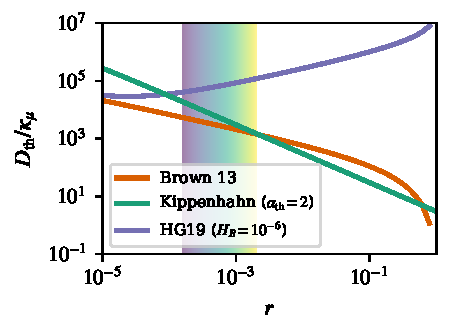
\includegraphics[width=\columnwidth]{Nu_models_comparison.pdf}
    \caption{ {\bf{(Done)}}
    Prescriptions of the compositional diffusivity due to thermohaline mixing $D_{\rm th}$ normalized by the molecular diffusivity $\kappa_{\mu}$ are plotted against the reduced density ratio $r$. For each prescription, we use $\mathrm{Pr} = \tau = 10^{-6}$, consistent with the conditions in these regions of RGB stars.
    We plot two hydrodynamic models, the \citet{brown_etal_2013} model (orange) and the \citet{kippenhahn_etal_1980} model with $\alpha_{\rm th} = 2$ (green). In both cases, the mixing efficiency decreases with $r$.
    The \citet{harrington} model (HG19) is also shown; it includes magnetic fields, which cause mixing efficiency to increase with $r$ for these parameters.
    The plotted curve for the HG19 model depends on $H_B$, which depends on the stellar structure and magnetic field strength; the plotted value is characteristic of the structure in the thermohaline zone of a 1.1 $M_\odot$ star at [Fe/H] = -0.2 with a magnetic field whose strength is $\mathcal{O}(100 \,\mathrm{G})$.
    The purple-to-yellow color gradient plotted in the background denotes the range of $r$ values that we measure in our grid of 1D stellar evolution models, which are displayed in Fig.~\ref{fig:mesa_r_spread}.
    }
    \label{fig:parameterization_compare}
\end{figure}
